% Abstract for TOCE special issue on Learning analytics, Abstract due May 15
% Limit(?): 1000 words
% When is final paper due? And, do we get notification to be allowed to submit?

% v2-acmsmall-sample.tex, dated March 6 2012
% This is a sample file for ACM small trim journals
%
% Compilation using 'acmsmall.cls' - version 1.3 (March 2012), Aptara Inc.
% (c) 2010 Association for Computing Machinery (ACM)
%
% Questions/Suggestions/Feedback should be addressed to => "acmtexsupport@aptaracorp.com".
% Users can also go through the FAQs available on the journal's submission webpage.
%
% Steps to compile: latex, bibtex, latex latex
%
% For tracking purposes => this is v1.3 - March 2012

\documentclass[prodmode,acmtecs]{acmsmall} % Aptara syntax

% Package to generate and customize Algorithm as per ACM style
\usepackage[ruled]{algorithm2e}
\renewcommand{\algorithmcfname}{ALGORITHM}
\SetAlFnt{\small}
\SetAlCapFnt{\small}
\SetAlCapNameFnt{\small}
\SetAlCapHSkip{0pt}
\IncMargin{-\parindent}

% Metadata Information
\acmVolume{}
\acmNumber{}
\acmArticle{}
\acmYear{2016}
\acmMonth{5}

% Copyright
%\setcopyright{acmcopyright}
%\setcopyright{acmlicensed}
%\setcopyright{rightsretained}
%\setcopyright{usgov}
%\setcopyright{usgovmixed}
%\setcopyright{cagov}
%\setcopyright{cagovmixed}

% DOI
\doi{0000001.0000001}

%ISSN
\issn{1234-56789}

% Document starts
\begin{document}

% Page heads
\markboth{A. C. Bart et al.}{Learning Analytics in a Computational Thinking Data Science Course}

% Title portion
\title{Learning Analytics in a\\Computational Thinking Course on Data Science}
\author{AUSTIN CORY BART
\affil{Virginia Tech}
JAVIER TIBAU
\affil{Virginia Tech}
ELI TILEVICH
\affil{Virginia Tech}
DENNIS KAFURA
\affil{Virginia Tech}
CLIFFORD A. SHAFFER
\affil{Virginia Tech}}
% NOTE! Affiliations placed here should be for the institution where the
%       BULK of the research was done. If the author has gone to a new
%       institution, before publication, the (above) affiliation should NOT be changed.
%       The authors 'current' address may be given in the "Author's addresses:" block (below).
%       So for example, Mr. Abdelzaher, the bulk of the research was done at UIUC, and he is
%       currently affiliated with NASA.


%
% The code below should be generated by the tool at
% http://dl.acm.org/ccs.cfm
% Please copy and paste the code instead of the example below. 
%
\begin{CCSXML}
<ccs2012>
<concept>
<concept_id>10003456.10003457.10003527.10003528</concept_id>
<concept_desc>Social and professional topics~Computational thinking</concept_desc>
<concept_significance>500</concept_significance>
</concept>
<concept>
<concept_id>10003456.10003457.10003527.10003540</concept_id>
<concept_desc>Social and professional topics~Student assessment</concept_desc>
<concept_significance>300</concept_significance>
</concept>
<concept>
<concept_id>10010147.10010257.10010321</concept_id>
<concept_desc>Computing methodologies~Machine learning algorithms</concept_desc>
<concept_significance>100</concept_significance>
</concept>
<concept>
<concept_id>10010405.10010489.10010491</concept_id>
<concept_desc>Applied computing~Interactive learning environments</concept_desc>
<concept_significance>100</concept_significance>
</concept>
</ccs2012>
\end{CCSXML}

\ccsdesc[500]{Social and professional topics~Computational thinking}
\ccsdesc[300]{Social and professional topics~Student assessment}
\ccsdesc[100]{Computing methodologies~Machine learning algorithms}
\ccsdesc[100]{Applied computing~Interactive learning environments}

%
% End generated code
%

% We no longer use \terms command
%\terms{Design, Algorithms, Performance}

\keywords{Learning Analytics, Computational Thinking, Computing Education, Data Mining}

\acmformat{Austin Cory Bart, Javier Tibau, Eli Tilevich, Dennis Kafura, and Clifford A. Shaffer, 2016. Data Mining a Computational Thinking Course on Data Science.}
% At a minimum you need to supply the author names, year and a title.
% IMPORTANT:
% Full first names whenever they are known, surname last, followed by a period.
% In the case of two authors, 'and' is placed between them.
% In the case of three or more authors, the serial comma is used, that is, all author names
% except the last one but including the penultimate author's name are followed by a comma,
% and then 'and' is placed before the final author's name.
% If only first and middle initials are known, then each initial
% is followed by a period and they are separated by a space.
% The remaining information (journal title, volume, article number, date, etc.) is 'auto-generated'.

\begin{bottomstuff}
This material is based upon work supported by a grant from the National Science Foundation Graduate Research Fellowship, Grant No. DGE 0822220.

Author's addresses: Austin Cory Bart, Javier Tibau, Eli Tilevich, Dennis Kafura, and Clifford A. Shaffer, Computer Science Department,
Virginia Tech.
\end{bottomstuff}

\maketitle

\bigskip\bigskip

\section{Introduction}
%READY%

As students of all majors and career paths are now expected to learn about computing, computer science education is challenged by the unprecedented scale and complexity of the effort required to address this requirement.
Many institutions now offer courses in ``Computational Thinking'', which cover foundational computing concepts, including algorithm development, data abstraction, and computing ethics to educate diverse majors from the sciences, arts, humanities, and other fields.
Although the material covered may not be as rigorous or in-depth as traditional introductory computing courses, thinking computationally is often new for these students and they may suffer from low self-efficacy about their ability.
Further, as non-major students often fail to immediately appreciate how computing can benefit their long-term career, their resulting motivation level can prove insufficient to see them through the more challenging aspects of the curriculum.
Hence, courses that serve these students need to focus on both cognitive and motivational concerns.
Ideally, new techniques should be developed to identify which students are struggling as early as possible, so that interventions can be staged to rescue and guide learners.

In this paper, we introduce a new iteration of our take on a Computational Thinking course for undergraduate non-Computer Science majors.
We have previously reported on an earlier version of this course in an ItiCSE paper~\cite{kafura2015design}, but with an emphasis on the tools and curriculum designed rather than on assessments and course outcomes.
Not only have we iterated upon the design of the course, but we have improved the instrumentation during the semester to collect fine-grained data about our learners.
In this paper, we expand on the nature and mechanics of the course and explore the results of learning analytics collected during the latest offering.
Our goal is to establish ground truth for the various outcomes of our course, in terms of motivational, engagement, and cognitive.
These outcomes have previously been based on educational theory rather than driven by the results of data collection.
We also seek to find whether these outcomes can be predicted earlier in the course, in order to identify at-risk students -- we report on some initial approaches in this avenue.
Finally, we review the needed changes for our course.

\section{Background}
%READY%

Both the design and evaluation of our course has largely been driven by theory.
The course material is based on work in the subfield of Computational Thinking, with a number of notable divergences.
The pedagogy and structure of the course is informed by educational theories such as Situated Learning Theory, Active Learning, and Instructional Design.
Finally, our evaluation is modeled after similar efforts in the Computing Education Research literature.

\subsection{Computational Thinking}
%READY%

When we first started designing our course to teach ``Computational Thinking'', we felt it was essential to precisely define the material we would cover.
Unfortunately, there is still limited consensus on \textit{what} exactly CT is, how it should be taught, and how to assess learner's understanding.
An excellent resource for summarizing the history of Computational Thinking research is the 2013 dissertation by Wienberg~\cite{weinberg2013}. 
The term ``Computational Thinking'' was coined by Seymour Papert in 1993~\cite{papert1996} and popularized by Dr. Jeannette Wing's 2006 paper~\cite{wing2006}. 
Wineberg's comprehensive survey analyzed 6906 papers directly or indirectly related to Computational Thinking that emerged after Wing's paper.
Their summary particularly criticizes the existing research for a lack of assessment and evaluation, with few papers reporting an operational definition of computational thinking (and many of those simply describing computational thinking as a ``way of thinking'', a ``fundamental skill'', or a ``way of solving problems'').

In the past decade, a number of initiatives have established learning objectives to attempt to describe computational thinking~\cite{google-computational-thinking,csta-computational-thinking}, incorporating a range of topics.
Our particular definitions (given more concretely later in section \ref{sec:course-content}) are distilled from these objectives, focusing on Abstraction (representing real-world objects with quantifiable properties), Algorithms (manipulating those properties with concrete instructions), and the Social Impacts of computing (relating the implications and interpretations of computations to stakeholders and society).
We chose these three particular key learning objectives in order to keep our core learning objectives simple and provide a clear overarching message to students.
Besides our chosen learning objectives, we also diverge from much of the literature by choosing to focus on undergraduate education instead of K-12.

\subsection{MUSIC Model of Academic Motivation}
%READY%

A major concern of the instructors was that students entering a course on Computational Thinking would have low levels of motivation.
To better understand the complex nature of motivation, we rely on the MUSIC Model of Academic Motivation to describe the dangers and opportunities of motivation~\cite{jones-description}.
The MUSIC Model is derived from a meta-analysis of other theories of motivation, incorporating only the academically relevant components, resulting in a theory that is useful for both designing and evaluating courses.
There are five key constructs in the MUSIC model:
\begin{description}
	\item[eMpowerment:] The amount of control or agency that a student feels that they have over their learning (e.g., course assignments, lecture topics, etc.).
	\item[Usefulness:] The expectation of the student that the material they are learning will be valuable to their short- and long- term goals, especially for their career.
	\item[Success:] The student's belief in their own ability to complete assignments, projects, and other elements of a course with the investment of a reasonable, fulfilling amount of work.
	\item[Interest:] The student's perception of how the assignment appeals to situational or long-term, individual interests. The former covers the aspects of a course related to attention, while the latter covers topics related to the fully-identified areas of focuses of the student.
	\item[Caring:] The students perception of other stakeholders' attitudes toward them. These stakeholders primarily include their instructor and classmates, but also can be extended to consider other members of their learning experience (e.g., administration, external experts, etc.).
\end{description}

Students are said to be motivated when one or more of these constructs is sufficiently present, as perceived by the student.
The MUSIC model has been relatively under-applied in Computing Education Research, compared to particular sub-theories involving subjects such as self-efficacy or interest; we felt that when designing a course for non-majors, however, it was important to measure and build for all five components as much as possible.
We revisit the MUSIC model when designing our evaluations of students' motivation within the course, relying on our instruments rather than the existing ones.

\subsection{Situated Learning Theory}
%READY%

A learning experience is a complex sequence of contextualized events, and Situated Learning Theory can help guide and explain the structure of this experience.
Situated Learning Theory, originally proposed by Lave and Wenger, argues that learning normally occurs as a function of the activity, context, and culture in which it is situated~\cite{lave-situated}.
Therefore, tasks in the learning environment should parallel real-world tasks, in order to maximize the \textit{authenticity}.
The key difference is that learning is driven by the problem being solved, rather than the tools available.
Therefore, the problem being solved should lead directly to the tool being taught.
Contextualization is key in these settings, as opposed to decontextualized (or ``inert'') settings.
SL Theory separates the concepts of the course Content from the course Context.

The original work in Situated Learning Theory was not about pedagogy or instructional design. It simply described how people learn and the importance of context and collaboration, but did not recommend a particular teaching style.
Subsequent research by Brown \cite{brown1989situated} and others expanded the theory so that it could be applied to the design of learning experiences.
These expansions often naturally dictate the use of active learning techniques, reducing the role of lecture in favor of collaborative, problem-based learning activities.
There is also a strong emphasis on authenticity in assessment.
Choi \& Hannafin \cite{situated-cognition} describe a particularly useful, concrete framework for designing situated learning environments and experiences.
The Choi \& Hannafin framework has four key principles: the Context, described as the ``... The problem's physical and conceptual structure as well as the purpose of activity and the social milieu in which it is embedded''\cite{rogoff1984everyday}; the Content, the information intending to be conveyed to the students; Facilitations, the modifications to the learning experience that support and accelerate learning (commonly done through Scaffolds); and Assessment, the methods used to evaluate the learning experience and measure the progress of the student.

Based on SL Theory, we felt it was important to determine a suitable context for the course that would align with our course content.
As part of the overarching goal to bring more students into Computer Science, a large number of contexts have been explored in Introductory computing. 
The context of a learning experience grounds the learner in what they already known, in order to teach the new material.
Some introductory computing experiences focused on presenting the content as purely as possible, which can come across as abstract and detached~\cite{Zografski}.
However, starting with Seymour Papert's work with robotics and the LOGO programming environment in the 70s~\cite{papert1996}, instructors have been interested in motivating students' first experience with richer contexts.
Some of these contexts rely on Situational Interest (e.g.,  Digital Media ``Computation'' ~\cite{guzdial-media-comp} and Game Design~\cite{Zografski}), while others attempt to provide enduring career value (e.g., [Big] Data Science ~\cite{Anderson}) and  social applicability (e.g,. Problem Solving for Social Good~\cite{SocialGoodinComputingEducation}).
When designing our course, we felt these last two contexts would be able to support the largest range of introductory learners while aligning with our course content.

\subsection{Peer Instruction}
%READY%

One of the more compelling and consistent results in Computer Science education is the effectiveness of peer instruction techniques~\cite{peer-instruction}.
Many studies and theories suggest that students learn more and become more motivated in courses that allow structure collaboration~\cite{peer-instruction-motivation}.
Further, collaboration techniques can allow courses to scale more efficiently by reducing the burden on the course staff, as students have more human resources to draw upon.
Finally, the diversity of students in the course can be leveraged to help students better understand how computing is used across different fields.

\subsection{Instructional Design}
%READY%

% Strongly considering deleting this section

In our later iterations of the developed course, our approach has been informed by formal methods of Instructional Design.
Instructional Design is a subfield of education concerned with the development of instructional materials and strategies that are aligned with actual learner needs, similar to the benefits that software engineering brings to programming.
There are many models of Instructional Design, but most involve similar major concepts.
Crucially, best practices are to establish learning objectives first, then to develop assessments, and finally develop assignments from those assessments.
This promotes alignment between the objectives, assignments, and assessments.

After initial iterations of our course, we found a number of topics that the instructors felt that students struggled with.
To improve students' performance, we used the ID process to develop clear learning objectives and assessments to evaluate our assignments.
Our hope is that the data collected through these instruments will help us in refining the assignments.

\subsection{Learning Analytics in Introductory Computing}
%READY%

Learning Analytics and Educational Data Mining are interrelated fields concerned with tracking, organizing, and predicting student performance in order to achieve improved learning and other course outcomes.
Learning analytics and data mining cover a wide range of techniques.
In a recent paper, An ITICSE working group summarized the recent research in this area~\cite{Ihantola:2015}. 
The group suggests that very few pre-CS1 courses have been analyzed (11\%), even though they also include high school courses in that number.
Further, they note that very few papers looked at Python-based courses, compared to Java courses.
They compare and contrast the different statistical approaches and techniques used by the various authors; in the context of this paper, we rely largely on descriptive, detailed, and exploratory types of statistical analyses, in addition to other types of computational analyses (e.g., log analyses, program analyses).


\section{Course Components}
%READY%

Although there are a number of existing Computational Thinking curricula, we have defined a particular set of educational objectives and course topics that we believe are valuable for our students.
This means that large portions of our course were created from scratch to achieve our pedagogical goals.
To support this, we have created a range of innovative technological scaffolding and apply modern pedagogical techniques (e.g., peer instruction, active learning, etc.) that enable us to capture and catalog a large quantity of learning analytics to guide course development.
In this section, we describe the courses' audience, content, context, structure, technology, and assessments.

\subsection{Audience}
%READY%

Our Computational Thinking curriculum was designed to fulfill new general education requirements at our university, providing ``Computational Thinking'' to all undergraduates.
Therefore, students will come from the arts, social sciences, humanities, agriculture, and more.
Although some sciences and engineering majors enroll, it is expected that most students will largely not be STEM majors.
In fact, students are expected to have no prior programming experience, and the course itself has no prerequisites.
The course is intended for any year, from Freshman to Senior.

\subsection{Course Content}
%READY%

\label{sec:course-content}

The three major topics in the course are:
\begin{itemize}
\item \textbf{Abstraction:} The idea that real-world entities (e.g, people, objects, events, actions, processes, etc.) can be simplified and concretely represented to suit the needs of some stakeholder.
\item \textbf{Algorithms:} The idea that computational abstractions can be manipulated using formal language.
\item \textbf{Social Impacts:} The idea that computing provides new powers and knowledge that can influence society.
\end{itemize}

Our core learning objective is for students to be able to create an algorithm that manipulates and processes data into a shape that can be used to answer real-world problems.
Students must express their algorithms using a practical programming language -- in this case, Python.
Further, they must be able to navigate and describe data in contexts related to their own careers and across other fields.
Finally, they should be able to discuss the social impacts, relevant stakeholders, and ethics of the questions and answers they find.

Figure \ref{fig:fundamental-elements} illustrates the hierarchical and connected nature of two of the courses' topics, Algorithms and Abstractions.
Algorithms, fundamentally, describe \textit{actions} in a specific \textit{sequence}.
Depending on the formality of the algorithmic agent, these actions can vary in complexity and atomicity. 
Higher-order constructs empower algorithms with the ability to branch (make \textit{decisions}) and repeat (\textit{iterate}).
Abstractions are concretely represented as variables or \textit{properties}, which formally have \textit{types} and quantitative characteristics. 
We refer to variables as properties to avoid confusing students with the algebraic term.
Higher-order organizational structures such as homogeneous \textit{lists} and heterogeneous \textit{dictionaries} allow for more efficient navigation of complex data.
Connecting these two ideas is \textit{state}, actions manipulating properties over the course of executing a program.
Taken together, these concepts describe our ideal ``notational machine'' for students, unifying their understanding of control structures with the data structures being manipulated.

In the original version of the course, we also taught a unit on creating functions to encapsulate reusable bits of code.
However, time restrictions forced us to remove those lessons.
Instead, modules and functions are introduced as mechanisms for reusing existing code written by other developers, without any lecture time devoted to creating functions.
In many cases, we attempt to provide this material on functions in individual lessons with students.

\begin{figure}
\centering
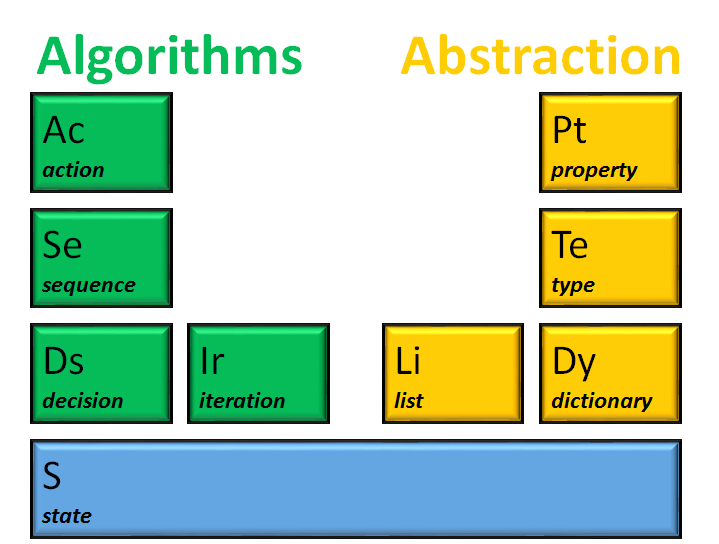
\includegraphics[width=.5\textwidth]{images/CTElements}
\caption{Fundamental Elements of Algorithms and Abstraction}
\label{fig:fundamental-elements}
\end{figure}

\subsection{Course Context}
%READY%

\label{sec:course-context}

In addition to the core course content, there is also a motivating context of Data Science: extracting meaning from data using computational analyses.
Our argument to students is that most disciplines benefit from data science, since the world is becoming increasingly data-driven.
To that end, we have collected a large repository of datasets that can appeal to a wide range of majors (discussed further in \ref{sec:CORGIS}).
Students use these datasets to create visualizations (e.g,. histograms, line plots) and perform simple statistical calculations (e.g., average, maximum, counts).
These kinds of analyses, while not particularly statistically rigorous or computationally difficult, provide a range of appropriate introductory-level problems.
They are tasked with interpreting these visualizations in a social context, further supporting the core learning objectives.

\subsection{Course Structure}
%READY%

There are several distinct phases to the course: the introduction, hands-on conceptual activities, BlockPy, the Mini-project, and the Final Project.

%\begin{tabular}
%Module & Topic \\
%\end{tabular}

\begin{figure}
\begin{tabular}{c | l | l | r}
Module & Topics & Time Period \\\hline
1 & Course Overview & Days 1-4 \\
2 & Computational Modeling and Abstraction  & Days 5-9 \\
3 & Algorithms and Programming & Days 10-14 \\
4 & Python and Big Data &  Days 15-19 \\
5 & Mini-project & Days 20-22 \\ 
6 & Final project & Days 23-29 \\
\end{tabular}
\end{figure}

Module 1 is a brief overview of the course, walking through the major topics and the cohort system. After their introduction to 
the course, they are tasked with using NetLogo \footnote{https://ccl.northwestern.edu/netlogo/} and then the Blockly Maze game \footnote{https://blockly-games.appspot.com/maze}.
These two applications respectively introduce the overarching ideas of Abstraction and Algorithms.

In Module 2, they begin learning fundamentals of working with computational abstractions and basic control structures, working mostly with paper-and-pencil and kinesthetic activities.
In one lesson, cohorts work together to write instructions for a ``card-sorting robot'', executed by the course staff on playing cards in order to demonstrate the basics of algorithm design and the ambiguities of natural language.
The course staff also performs a ``Play'' that models the state of the program, the program counter, and console for a simple algorithm to process a list of data; during the execution of the program, the instructor regularly stops the lesson and has students predict the next state.
There are also a series of smaller pencil-and-paper activities for topics relating to decision, iteration, and abstraction.

During Module 3, students must complete a series of programming assignments in BlockPy, a block-based programming environment for Python.
These assignments incorporate real-world datasets from the CORGIS project, and students are tasked with creating charts and computing simple statistical information (averages, counts, thresholds, etc.).
By the end of Module 3, they are expected to be working in the ``text mode'' of BlockPy, to prepare them for the transition to Module 4.
This next module builds on their Python experience by having them complete similar programming assignments, except this time in a professional desktop IDE named Spyder \footnote{https://pythonhosted.org/spyder/}.
They will continue to use Spyder in Modules 5 and 6, where they complete a Mini-project and their final project. 
During the Mini-project, students work in their cohort to answer questions about the CORGIS State Crime dataset; as a group, they create visualizations and a presentation, which they are individually responsible for presenting as a video.
This is largely practice for their final project, which is a month long individually-paced activity to create a 5-minute video presentation answering questions related to a dataset of their choosing using python-based visualizations.

Throughout the course, most of the modules end with a day on Social Impacts.
In the first module, students review final projects from previous semesters that are relevant to their career interests and must discuss and critique the social impacts of the video.
In the second module, students watch a video about an ethical scenario where a computer potentially caused an accident, and they are asked to debate within their cohorts the ethical ramifications. 
The third module ends with a brief lesson about various ethical frameworks (e.g., Utilitarianism, Duty, Common Good, etc.) and then to apply these frameworks to the debate from the previous module. 
In both the mini-project and the final project, students are expected to discuss the social impacts of the questions and answers that they determine. 

Throughout the course, students are also tasked with daily readings accompanied by reading quizzes.
The readings, written specifically for the curriculum by the course staff\footnote{http://think.cs.vt.edu/book/}, introduce the material for the day with a few pages of prose and images.
These quizzes are short, multiple-choice assignments that are expected to take only a few minutes.
They are administered and automatically graded by Canvas.
Students are allowed 3 attempts before the quiz closes

The class meets twice a week for 75 minutes.
A typical day of the course begins with an introductory lecture on the material.
Students then work in their cohorts or individually to complete the interactive component (e.g., paper-and-pencil activity, collaborative discussion, programming assignment, project work).
Finally, the class comes back together to discuss the lessons of the day and any challenges that occurred.
Most lessons also include a required homework unit meant to reinforce students' learning and prepare them for the next class.

\subsubsection{Cohorts}
%READY%

On the third day of the course, students are grouped into collaborative cohorts of 5-6 students.
Each undergraduate teaching assistant (UTA) is responsible for two cohorts.
A graduate teaching assistant is responsible for managing the UTAs, and in turn is overseen by the course instructors.

Most early classwork activities are explicitly collaborative, and students are expected to generate a single answer for their cohort.
During the programming assignment section of the course, most assignments require individual submissions, but students are allowed work together and get help.
Students are forbidden from sharing their solutions, but are encouraged to share their thought process and provide support.
Near the end of the course, students complete a group ``Mini-project'' to prepare for their individual Final project. This mini-project allows a cohort to create questions and visualizations collaboratively, although they are individually required to submit their own presentation.

\subsection{Course Technology}
%READY%

To support our learners, we use a variety of educational technology to scaffold their learning, including a Learning Management System, an introductory programming environment, and specially prepared dataset libraries.
The activities that students complete in the course, along with surveys, teacher observations, and interaction logs, provide a rich data source for our research questions, and their collection is facilitated by these libraries.

\subsubsection{Canvas}
%READY%

Although the course met twice a week in person, much of the course material was disseminated through the Canvas Learning Management System.
In previous iterations of the course, we used a custom platform named Rhinestone~\cite{kafura2015design}, based off the Runestone project.
Although Rhinestone gave us a tremendous amount of flexibility in developing the prototypical versions of our course, we felt that this would cause maintenance issues in the long-term.

Canvas supports the Learning Tool Interoperability (LTI) standard, so that more sophisticated tools can be embeded in the learning platform. 
The class readings were stored as Pages, which enabled us to embed interactive BlockPy canvases.
Assignments could integrate BlockPy problems.

\subsubsection{BlockPy}
%READY%

In their first exposure to programming, students use a block-based environment (BlockPy) with automatic, guiding feedback.
BlockPy features a dual, bidirectional blocks-to-text coding interface that is heavily instrumented, constantly recording user interactions and code.
This environment facilitates the students' transition into Python during the last part of the course, yielding a more authentic programming experience.
BlockPy also integrates both real-world datasets (e.g., weather data, stock trading data) and tools for generating visualizations (e.g., line plots).
Another major feature of BlockPy is the State Explorer, which visualizes the value of variables as they change over the course of the program.

BlockPy supports the LTI standard in order to integrate with Canvas, allowing instructors to embed interactive workspaces and assignments within their courses.
Students are free to work on an assignment until it is completed.
Grades are passed back to Canvas upon completion.

\subsubsection{CORGIS}
\label{sec:CORGIS}
%READY%

Throughout the course, students use datasets specially designed and scaffolded for introductory computing students with data drawn from diverse, real-world sources relevant to their diverse majors (e.g., supreme court decisions, historical slave sales, incidences of diseases across the country, real-time weather forecasts, etc.).
To make data conveniently available to students, we use the CORGIS (Collection of Really Great and Interesting dataSets) Project.
The CORGIS project makes over 40 datasets available as both raw datasets and convenient language bindings.
We use the Python language bindings and allowed students to choose their own dataset.

\subsection{Assessments}
%READY%

Our final assessment of students is a month-long project where they individually apply Computational Thinking to answer questions relevant to their own major.
Students use a dataset of their own choosing, write algorithms to process and visualize the data, and then create a detailed, video report on their findings.
Students are evaluated using a rubric on the quality of their report across several metrics, including the quality of their questions, their ability to explain their data abstractions, and the social impacts of their results.
The programs that students create during this process are also evaluated, and the students are expected to explain automatically-extracted segments of their code using technical vocabulary.
These two sources of data serve as ground truth of their Computational Thinking ability.

When developing the course, the instructors wanted to have the final assessment be as authentic as possible. Therefore, students are assessed through a 5-week final project where they conduct their own computational analysis of an existing data source related to their career interests.
They begin by choosing a data source from our collection.
Then they form preliminary questions that could conceivably be answered using the dataset.
They construct a ``map'' of their dataset to help them navigate its structure and to become more familiar with the individual fields.
They then write programs to process the data and create visualizations that will answer their questions.
They are encouraged to refine their questions as they learn more about their data source.

Students are assigned a final grade that is calculated based on their attendance, performance on classwork and homework, their completion of reading quizzes, and their final project scores. The weighting heavily favors effort-based work, such as their classwork and homework, but also includes their final project score quite heavily.

\section{Data Collection}
%READY%

\begin{figure}
\centering
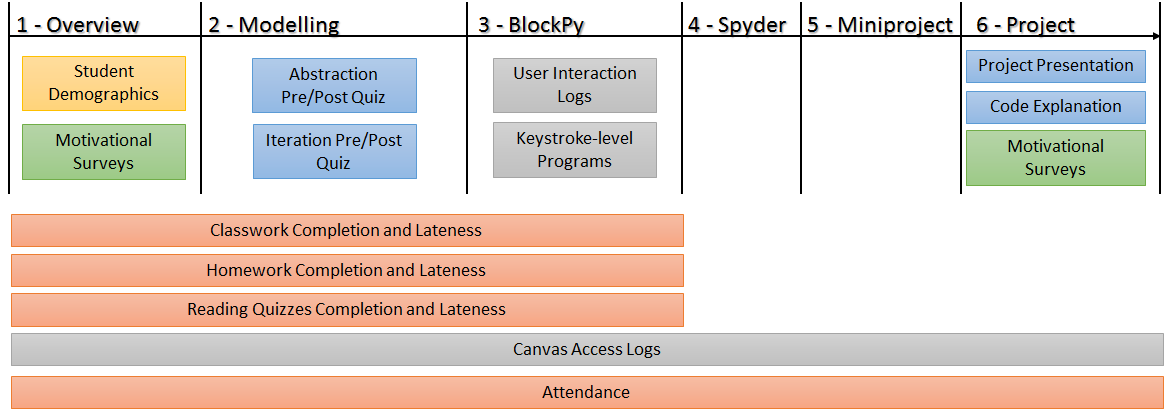
\includegraphics[width=\textwidth]{images/timeline}
\caption{Data Collection Timeline}
\label{fig:timeline}
\end{figure}

All data was collected with full compliance from our Institutional Review Board.
Students were informed that data would be collected from the various computational tools.
Consent was gathered using paper release forms. Only 1 student did not give consent to the use of her data, and so her data was removed.
After collection, all data was anonymized, and will only be reported in aggregate.

\subsection{Abstraction and Iteration Quizzes}
%READY%

Two topics that the course staff felt students particularly struggled with were Abstraction and Iteration.
In the spirit of Instructional Design, the staff developed two lessons that would particularly target these topics.
They began the process by identifying the key learning objectives for these topics, and using them to generate brief, 8-question pre/post quizzes that would wrap the lesson.
Theses quizzes would be used to measure students initial and final understanding of the topics, but also their learning gains.

\subsection{Final Project}
%READY%

As previously described, the final project for the course is a month-long project where students use a dataset related to their career interests to conduct a computational analysis and answer questions.
Once they have developed answers to their questions, students create a 5 minute video presentation (e.g. by using PowerPoint).
This presentation is assessed using an 8-item rubric, which they are encouraged to reference while they are developing the presentation.
The components of the rubric are as follows:
\begin{description}
    \item[Abstraction] What is the relationship between a real-world entity and the data?
    \item[Data Structure] How is data for the project organized? What fields in the data are particularly relevant to the stakeholder?
    \item[Questions] What questions were explored?
	\item[Visualizations] How did students graphically present the results of their analysis?
    \item[Answers] What were the answers to the questions? How does the student interpret them?
    \item[Limitations] What are limitations of the data provided, and the kinds of analyses that could be performed?
    \item[Social Impacts] Who is interested in the results of the analysis, and who is affected? What potential concerns or problems can arise with regards to the analyses' impact?
    \item[Communication] Were the slides well-constructed? Did the student convey them clearly?
\end{description}


\subsection{Code Explanations}
%READY%

In addition to the video, students' code is assessed using a special tool.
Figure \ref{fig-code-explainer} demonstrates the Code Explanation interface.
Students are prompted to upload one of their Python code files (whichever one has the most code, if a student has written more than one file).
The software constructs an Abstract Syntax Tree of the code and selects lines based on presupplied criteria.
In particular, the software attempts to find 5 lines with examples of the following code constructs:
\begin{enumerate}
    \item For loop (iteration)
    \item Assignment
    \item Dictionary access
    \item Appending to a list
    \item If statement (decision)
    \item Dataset module import
    \item Plot or Print statements
\end{enumerate}
These constructs are ordered from most desirable to least desirable, and selected greedily.
Five lines will always be chosen, even if a single line contains multiple constructs (e.g, a dictionary access inside of an append statement).
If a student submits a program with less than five lines, or with constructs present on less than five lines, all of the lines will be chosen.

The student is presented with the five lines, and charged with writing a 1-2 sentence explanation of the line using technical vocabulary.
One of the instructors of the course graded all of the code explanations using a checklist.
If a code construct was present in the sampled code, then students had an opportunity to gain or lose points based on correctly or incorrectly describing that construct.
For instance, an assignment statement presents an opportunity for students to describe the idea of storing or setting a variable, but also presents a risk for students who incorrectly suggest that the right-hand side of the assignment is affected by the left-hand side.
The complete rubric used for grading the code explanation activity is available in appendix %TODO: \ref{apx-explanation-rubric}.

\subsection{Surveys}
%READY%

Students were surveyed at the beginning and end of the course using 26 quantitative questions and 6 qualitative questions.
The quantitative questions were on a 7-point likert scale, from "Strongly Disagree" to "Strongly Agree".
The first 25 questions are a cross-product of the five core course components and the five previously described motivational aspects of the course (eMpowerment, Usefulness, Success, Interest, Caring).
For the purposes of our survey, we defined the five core course components as: learning to program (content), learning to work with abstractions (content), learning about social ethics of computing (content), learning to work with real-world data (context), working in cohorts (major scaffold).
So, for example, a student would be asked to rate their agreement with a statement such as, ``During the course, I felt that it was useful to my career to learn how to program'' or ``During the course, I felt it was interesting to learn about social ethics of computing''.
The 26th quantitative question asks students if they intend to continue to learn computing, either formally or informally.
In the end of semester survey, students were also asked a series of 6 questions relating to the success of their cohort.
These questions are based on a study done by Google that found a set of five major factors in the success of teams~\cite{google-teams}.
Therefore, these questions students' perceptions of their psychological safety within the cohort, dependability on their cohortmates, the structure and clarity of their assigned tasks, their perception of their cohorts sense of the usefulness of the work, and their cohorts helpfulness to themselves.

\subsection{Log Data}
%READY%

The course was embedded in the Canvas Learning Management System.
After the course was completed, we obtained a detailed log of all student page accesses.
This includes information not just about their time spent on course readings, but also their accesses of the assignment feedback pages.
Attendance was recorded and collected through a Canvas plugin by the Undergraduate Teaching Assistants on a daily basis. 

During the middle phase of the course, students use a web-based, dual block/text Python programming environment named BlockPy.
We have previously published a technical description and results from a classroom pilot for BlockPy in \cite{compsac-blockpy}. 
Students' interactions with with the BlockPy environment are logged at a fine-grained level. 

\subsection{Static Analysis}
%READY%

Python is a dynamic language that only gives run-time errors, as opposed to static errors. To extend our analysis of students' code, we wrote a flow-sensitive static analyzer to perform some simple analyses.
Although flow-sensitivity is usually computationally prohibitive, the analyzer takes advantage of the short, simplistic nature of the types of solutions present in the course; programs are typically less than 10 lines long and have little branching control flow.
This system can detect a range of of ``semantic errors'' that we have anecdotally observed in students code:

\begin{itemize}
	\item \textbf{Unread variables:} A variable was created but never read from, typically because a student was copying code blindly from another source.
    \item \textbf{Undefined variables:} The code attempts to read from an undeclared variable; a runtime error was avoided by guarding the read in an unexplored control flow path (e.g., empty for loop).
    \item \textbf{Overwritten variables:} A variable was written to and then written to before it could be read from; the first write was therefore redundant.
    \item \textbf{Used iteration list inside body:} The iteration list (the list being iterated upon in a foreach loop) was used within the body of the foreach loop, as opposed to the iteration variable. This is never used in the types of programs students were writing, and reveals a systematic misunderstanding of the nature of iteration.
    \item \textbf{Did not use iteration variable inside body:} Similar to the previous problem, students will also not use iteration variable inside the body, which is only appropriate for a small subset of problems (i.e., counting).
    \item \textbf{Reused iteration list for iteration variable:} Although not really an error, the student has chosen the same variable name for both the list and iteration variable (e.g., \texttt{for dogs in dogs} or \texttt{for dog in dog}).
    \item \textbf{Attempted to iterate over a non-list:} An integer or string variable was iterated over instead of a list.
    \item \textbf{Iterated over an empty list:} Students often create empty lists when performing filter or mapping operations, and would sometimes be confused about iterating over the existing list vs. the new list.
    \item \textbf{Changed the type of a variable:} A variable initially declared to be of one type is assigned a value of a different type.
\end{itemize}

The occurrences of these errors in students final submitted solutions is tabulated for each student and divided by the number of completed problems, in order to give a Semantic Error Rate (SER).

\section{Research Questions}
%READY%

Our primary research question is to determine which analytics can be used early in the course to predict student performance at the end of the course with regards to our cognitive, motivational, and engagement objectives.
With these predictions, we can answer our secondary research question: how one can design new interventions that can guide more students to success?
These interventions can be remedial lessons that target particular misconceptions, recommended interactions with the teaching assistants or professors, and improvements to tools to enhance the support students receive.
Our third and last research question is to determine what patterns of behavior are common among students in the course, and to identify and cluster students based on these patterns using data mining techniques.

\subsection{Demographics}
%READY%

53 students were enrolled in the course after the first two weeks, although by the end of the semester, 47 students received a passing grade.
Students were mostly Sophomores (35\%) and Juniors (31\%), with only 19\% Seniors and 14\% Freshmen; this represents a roughly normal distribution of ages averaged midway through college. 
The class was largely balanced by gender with 46\% female and 54\% male.
No students reported prior programming course experiences (i.e. college or high-school level courses).
Building Construction was easily the most over-represented major, with 36\%, followed by English with 17\%. Most other majors only had 1-3 students present and represented a very broad slice of the university: Public Relations, Political Science, Theatre Arts, International Studies, Biochemistry, and so on.
However, the college of Liberal Arts and Sciences had the largest share of colleges at 49\%.
Cohorts had 5-7 students in them, and each UTA was responsible for 11 or 13 students.

\subsection{Course Performance}
%READY%

Figure \ref{fig:final-project-subscores} shows the distribution of rubric grades for the 8 components of the final project presentation.
Although most of the class performed well across the components, there are noticeable deficiencies.
In particular, there were a large percentage of students who utterly failed to describe the Abstractions used in their project, and a similar non-trivial percentage who struggled with describing the structure of their data.
There are also very few students who scored ``Excellent'' at describing their Questions and Abstractions.

\begin{figure}
\centering
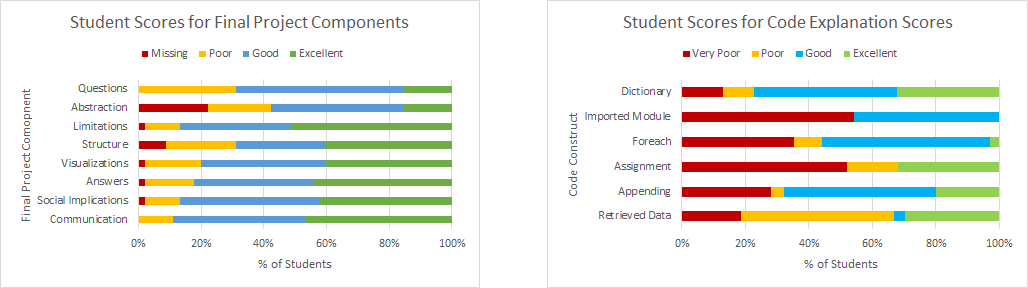
\includegraphics[width=\textwidth]{images/FinalProjectPerformance}
\label{fig:final-project-subscores}
\caption{Student Performance on the Final Project and the Code Explanation}
\end{figure}

Performance on the code explanation activity was relatively worse.
Overall, students were unable to use technical vocabulary to describe their code, and made a number of mistakes when doing so.
For instance, one student referred to ``if loops''.
In general, the only topics students performed well on were explaining dictionary access and append statements.
It is somewhat unsurprising that students performed so poorly with regards to explaining module imports and data retrieval function calls, since they were relatively understated in the course material.
However, it is very disappointing to see the students' very mixed performances for students' explanations of foreach loops and assignment statements, considering that these represent rather fundamental course topics (iteration and program state).
One consideration, however, is that the code explanation rubric is less developed than other course components, making it a very raw instrument for determining student ability.

The analysis revealed that the Visualization and Answer component of the Final Project rubrics are possibly redundant to each other, due to their very high correlation (.642**) and interrelated content.
Although there are a number of correlations between the scores for different code explanation constructs (Assignment was strongly statistically significantly correlated with Appending at .658** and with Foreach at .587**), we suggest it is less likely that the instrument has redundancy and more likely that it is measuring the same underlying skill to explain code, given the difference in the nature of the constructs.

All students had an SER above 1, suggesting that semantic errors were common for all students.
The distribution was roughly normal, with an average of 1.79 and standard deviation of .415.
Students' code explanation scores had a modest correlation with their SER (-.346**), suggesting a connection between students' ability to write semantically correct code and to explain that code.
There were no significant differences between demographic information and SER.

\subsection{Outcome Ground Truth}
%READY%

In our course, we consider a number of cognitive, motivational, and engagement outcomes.
The major cognitive outcomes for the course are related to the final project: their video presentation and their code explanations.
We are also interested in their performance on the Abstraction and Iteration quizzes, both in terms of final score and learning gains.
On the motivational side, we used the responses from the beginning and end-of-course surveys to measure students' self-reported motivation.
Finally, in terms of engagement, there are a number of different outcomes: attendance, number of late assignments submitted, the amount of time spent in the Canvas system, the amount of time spent working on BlockPy questions, and the quantity of classwork, homework, reading quizzes, and BlockPy questions completed.

We found a moderate, significant correlation (.510**) between students' presentation grades and their code explanation grades.
It would appear that students who perform well on the final project also tend to be able to explain the code associated with their project.
We find this to be a promising result, since it suggests some connection with these two different outcomes.

There were modest correlations between students' code explanations scores and their score on the Abstraction (.376*) and Iteration (.394*) post-quizzes; there were no significant correlations between these quizzes and the students project scores, however.
This suggests some separation from students understanding of algorithmic and programming concepts versus the skills demonstrated by their project presentation.

There were no significant correlations between students' performance on the abstraction quizzes (either the before or after) and their performance on the Abstraction on the component of the final project.
This suggests a serious misalignment between these two sets of instruments.

\subsection{Engagement Outcomes}
%READY%

Students' attendance was highly correlated with their completion of modules 1-4 (.597**), which suggests that, unsurprisingly, the students that show up to class get more work done.
Interestingly, there was a negative correlation between attendance and students perception of the usefulness of learning computing ethics to their career (-.342*) -- possibly, suggesting that some students may have intentionally avoided the ethics material.
Another negative (albeit weak) correlation occurred between attendance and students' perception of how useful their cohort-mates thought the material was (-.343*). 

One of the strongest correlations between the survey results and other course engagement outcomes is the high correlation between their completion of modules 1-4 and students' perception of how much course instructors cared that they learned to work real-world data (.406*).
Note that most other survey responses did not correlate strongly or significantly with their completion of the modules. 
It is curious that their sense of the instructors caring is the highest correlated, but overall suggests a theme that students perceived the course context very strongly during the modules.

Students self-efficacy to writing programs was moderately correlated with their completion of BlockPy problems (.397*).  
Students total time spent working on BlockPy problems was negatively correlated with two different survey responses: their intent to continue learning computing (-.369*) and their perception of how useful their cohort-mates thought the material was (-.443**).
The former might suggest that students who were interested in continuing might also be the students who can complete problems faster; the latter is more difficult to explain, but a potential hypothesis is that an implicit social pressure effect occurs where, if students believe that their peers undervalue the material, then they will devote less time to it.

Analyzing the start of semester surveys gives far less information.
The only strongly significant correlation was between students' self-efficacy to work with real-world data and their overall completion of reading quizzes (.451**).

\subsection{Demographics and Outcomes}
%READY%

A one-way ANOVA test was conducted between genders across the outcome variables established in previous sections.
There were no significant differences between genders for cognitive outcomes such as final project score, code explanation scores, or any of the quizzes.
However, engagement outcomes were another story.
Women had significantly more BlockPy coding sessions where they worked for at least 15 minutes on a problem ($49.96 \pm 16.49$ sessions), median session lengths when in Canvas ($14.99 \pm 7.15$ hours), higher completion rates of assignments ($1.07 \pm .47$ assignments), and higher attendance ($3 \pm 1$ days).
However, it is worthwhile to note that there were no differences between genders in any of the results of the motivation surveys, with the exception of students' perception of their empowerment to work with data of their own choosing (which women very weakly rated higher than men, at a $\alpha < .05$ level).
One-way ANOVA tests were also used to compare student years and course outcomes, but there were no significant differences across years

\subsection{Cohorts and Outcomes}

Another research question is whether cohorts have an impact on outcomes.

A one-way ANOVA test was performed between the cohorts and the following outcomes.
However, it appears that there are no significant differences between cohorts' performances.

Students received feedback through canvas.
UTAs were distinguishable very strongly by the amount and frequency of their feedback to students.
However, there were no statistically significant correlations between amount of feedback received and course outcomes.
Analyses reveal that most students did check the feedback.

\subsection{Predicting Outcomes}
%READY%

A major research goal was to establish what outcomes could be predicted at the beginning of the semester.
Student log data from the first two weeks and first month were analyzed, with students grouped into "above average" and "below average" levels. One-way ANOVA tests against course outcomes were used to identify significant predictable outcomes.

Students who loaded an above average number of Canvas Pages (which stored the course textbook) in the first two weeks had significantly more completed assignments ($1.20 \pm .485$ assignments).
Students who loaded the gradebook an above average number of times in the first two weeks also had significantly more completed assignments ($1.30 \pm .455$).
Both of these outcomes also had significance in the Final Course Grade, most likely because the Final Course Grade score is heavily based on the number of completed assignments.
However, students who loaded the feedback for individual assignments an above average number of times in the first two weeks scored significantly higher on the Final Course Grade ($6.17 \pm 2.65$ points) but did not complete significantly more assignments.
These three outcomes suggest that students who were conscientious about their classwork grades and readings were able to consistently complete more of their classwork.

Students who loaded the feedback for individual assignments an above average number of times in the first two weeks also had significantly longer median session lengths in BlockPy ($2.65 \pm .98$ minutes). Above average Page accesses and Submission checks in the first two weeks were also strongly associated with total BlockPy session length ($1.61 \pm .679$ hours and $1.57 \pm .653$ hours, respectively).

Completing an above average number of classwork assignments in module 1 (the first two weeks) was associated with a number of improved course outcomes.
Divided into these two groups, roughly one-quarter of the class did not complete all of the work in the first module; these students performed $13.9 \pm 5.13$ points lower on the final project.
Most importantly, these students scored roughly one level higher on the Abstraction component than students who did not.
Curiously, these associations did not carry over when module 1 and 2 were considered together. 
However, above average number of completed classwork assignments in modules 1 and combined was significantly associated with an increased intent to continue learning computing, at an increase of roughly one-half levels on the 7-point likert ($\pm$ half a level).

\subsection{Iteration and Abstraction Quiz}

Students improved measurably between both the abstraction and iteration quiz.
In fact, on both assessments, a matched-paired t-test suggests that class average went up a full point (out of the 8 points possible).

Reviewing the data, we found that students still struggled with a number of the concepts.

The simplest explanation is that the lessons were insufficient to teach the concepts.

However, the IRT analysis also revealed potential flaws in the quiz itself.
Although the iteration quiz questions had good levels of discrimination, the abstraction quiz questions were inferior.

\begin{figure}
\begin{tabular}{ l | c | c}
Instrument & Pre-quiz Cronbach's Alpha & Post-quiz Cronbach's Alpha \\\hline
Abstraction & .387 & .433 \\
Iteration & .293 & .430 \\\hline
Interest & .666 & \\
Useful & .808 & \\
Success & .825 & \\
Empowerment & .900 & \\
Caring & .889 & \\
\end{tabular}
\end{figure}

\section{Iterating the Course}

These data inform the next iteration of our course lessons and tools.

One of the biggest category of improvements are what automated tutor features can be added to the block-based programming environment to provide better guidance for beginner programmers---immediate, real-time feedback that can catch problematic behavior, correct students misconceptions, and forestall their frustration before it impacts their long-term course motivation.

We intend to integrate the static analyzer directly into the BlockPy environment, introducing a new class of error messages to students.

The first lesson on Abstraction in the course uses the NetLogo environment. 
In the original version of the course, the entire first module was oriented around using NetLogo.
However, as we increased the role of our block-based coding environment, the NetLogo piece became less and less relevant.
In this semester, we reduced students' time with NetLogo to a single day; in the next course offering, NetLogo will be completely replaced with a new interactive visualization tool that allows them to work with their final datasets.

In the second iteration of the course, we introduced a ``Mini-project'' to help prepare students for the final project.
Building on that success, we are now introducing a ``Micro-project'' and ``Nano-project''.
These projects grow incrementally through the course, as students increase their computational toolkit.
Our expectation is that 

A major limitation for scaling the course is the final project.
Students create a 5-minute video that must be graded against a rubric.
Presently, both teaching assistants and course instructors grade these videos at the end of the semester over a week-long period.
The instructors feel that it is important for students to have two layers of grading to ensure fairness and to account for variability across graders.
Although this is tractable for 50 students, it becomes an unbearable burden on the instructor for 100-500 students. 
A potential remedy for this is to move to a more probabilistic model.
UTAs will remain responsible for grading every one of their students, while instructors will grade only a sampling of each UTAs' students (perhaps a low grade, high grade, and medium grade).
The discrepancies between the UTAs and course staff can then be adjusted to normalize grades.
Further, a system for appealing grades could be instituted, so that students can ask the instructor to grade their project too -- with the understanding that the new grade might be less friendly.

\subsection{Planning Interventions}

Ideally, more assessments can be conducted throughout the course to gather more data on students' learning trajectories.

For example, the earlier abstraction and iteration quizzes could be repeated to determine if students retain their knowledge about these subjects.

\subsection{Planning Data Collection}

Another category is what types of data we are seeking to collect in future iterations, whether to rely more on course staff observations, automatic data logs, or the results of preliminary assessments.
We will also identify relevant learning analytics that Computational Thinking courses can use to measure and cluster students early, thus enabling adopters to implement our curriculum at-scale effectively.
Finally, we will identify common problematic patterns in students and potential solutions for supporting them that other tool developers could use to improve their environments.

\section{Threats to Validity}

The largest and most serious threat to validity is the relatively small course size (N=50 students).
We are actively expanding every semester, and we expect to double the number of enrolled students in the next offering.
In fact, long-term, we hope to scale this course to handle potentially hundreds of students every semester.

\section{Conclusions}

% Bibliography
\bibliographystyle{ACM-Reference-Format-Journals}
\bibliography{citations}

                             % Sample .bib file with references that match those in
                             % the 'Specifications Document (V1.5)' as well containing
                             % 'legacy' bibs and bibs with 'alternate codings'.
                             % Gerry Murray - March 2012

% History dates
%\received{February 2007}{March 2009}{June 2009}

% Electronic Appendix

\end{document}
% End of v2-acmsmall-sample.tex (March 2012) - Gerry Murray, ACM


